%%%%%%%%%%%%%%%%%%%%%%%%%%%%%%%%%%%%%%
% Multiplicative domain poster
% Created by Nathaniel Johnston
% August 2009
% http://www.nathanieljohnston.com/2009/08/latex-poster-template/
%%%%%%%%%%%%%%%%%%%%%%%%%%%%%%%%%%%%%%

\documentclass[final]{beamer}
\usepackage[scale=1.24]{beamerposter}
\usepackage{graphicx}			% allows us to import images

%-----------------------------------------------------------
% Custom commands that I use frequently
%-----------------------------------------------------------

\newcommand{\bb}[1]{\mathbb{#1}}
\newcommand{\cl}[1]{\mathcal{#1}}
\newcommand{\fA}{\mathfrak{A}}
\newcommand{\fB}{\mathfrak{B}}
\newcommand{\Tr}{{\rm Tr}}
\newtheorem{thm}{Theorem}

%-----------------------------------------------------------
% Define the column width and poster size
% To set effective sepwid, onecolwid and twocolwid values, first choose how many columns you want and how much separation you want between columns
% The separation I chose is 0.024 and I want 4 columns
% Then set onecolwid to be (1-(4+1)*0.024)/4 = 0.22
% Set twocolwid to be 2*onecolwid + sepwid = 0.464
%-----------------------------------------------------------

\newlength{\sepwid}
\newlength{\onecolwid}
\newlength{\twocolwid}
\setlength{\paperwidth}{841mm}
\setlength{\paperheight}{594mm}
\setlength{\sepwid}{0.024\paperwidth}
\setlength{\onecolwid}{0.22\paperwidth}
\setlength{\twocolwid}{0.464\paperwidth}
\setlength{\topmargin}{-0.5in}
\usetheme{confposter}
\usepackage{exscale}

%-----------------------------------------------------------
% The next part fixes a problem with figure numbering. Thanks Nishan!
% When including a figure in your poster, be sure that the commands are typed in the following order:
% \begin{figure}
% \includegraphics[...]{...}
% \caption{...}
% \end{figure}
% That is, put the \caption after the \includegraphics
%-----------------------------------------------------------

\usecaptiontemplate{
\small
\structure{\insertcaptionname~\insertcaptionnumber:}
\insertcaption}

%-----------------------------------------------------------
% Define colours (see beamerthemeconfposter.sty to change these colour definitions)
%-----------------------------------------------------------

\setbeamercolor{block title}{fg=ngreen,bg=white}
\setbeamercolor{block body}{fg=black,bg=white}
\setbeamercolor{block alerted title}{fg=white,bg=dblue!70}
%\setbeamercolor{block alerted body}{fg=black,bg=dblue!10}
\setbeamercolor{block alerted body}{fg=black,bg=white}


%-----------------------------------------------------------
% Name and authors of poster/paper/research
%-----------------------------------------------------------

%\title{\parbox[c]{38in}{Lineage diversification in the genus \textit{Solanum }L. (Solanaceae)}
%\parbox[c]{5in{\includegraphics[width=5in]{./logos/ICL_logo.PNG}}\\ \includegraphics[width=5in]{./logos/ICL_logo.PNG}}}
\title{Plant functional diversity and the biogeography of biomes in North and South America}
\author{Susy Echeverr\'ia-Londo\~no$^{1*}$, Brian J. Enquist$^{2}$, Danilo M. Neves2$^{2}$, Cyrille Violle$^{3}$ \& Andrew J, Kerkhoff$^{1}$}
\institute{\small (1) Department of Biology, Kenyon College, Gambier, Ohio, USA; (2) Department of Ecology and Evolutionary Biology, University of Arizona, Tucson, Arizona, USA; (3) Centre d'Ecologie Fonctionnelle et Evolutive (UMR 5175), CNRS, Universit\'e de Montpellier, Universit\'e Paul Val\'ery, Montpellier, France \\ *echeverrialondono1@kenyon.edu}

%-----------------------------------------------------------
% Start the poster itself
%-----------------------------------------------------------
% The \rmfamily command is used frequently throughout the poster to force a serif font to be used for the body text
% Serif font is better for small text, sans-serif font is better for headers (for readability reasons)
%-----------------------------------------------------------

\begin{document}
\begin{frame}[t]
  \begin{columns}[t]												% the [t] option aligns the column's content at the top
    \begin{column}{\sepwid}\end{column}			% empty spacer column
    \begin{column}{\onecolwid}
      
      \small
      \begin{block}{Introduction}
        
      \end{block}
      \vskip2ex
      
  		
  	\begin{block}{Aim}
		
	\end{block}
    \vskip2ex
      		
     \begin{block}{Methods}
    
	\end{block}

\vskip2ex

      		
      		\begin{figure}[h]
      			\centering
      			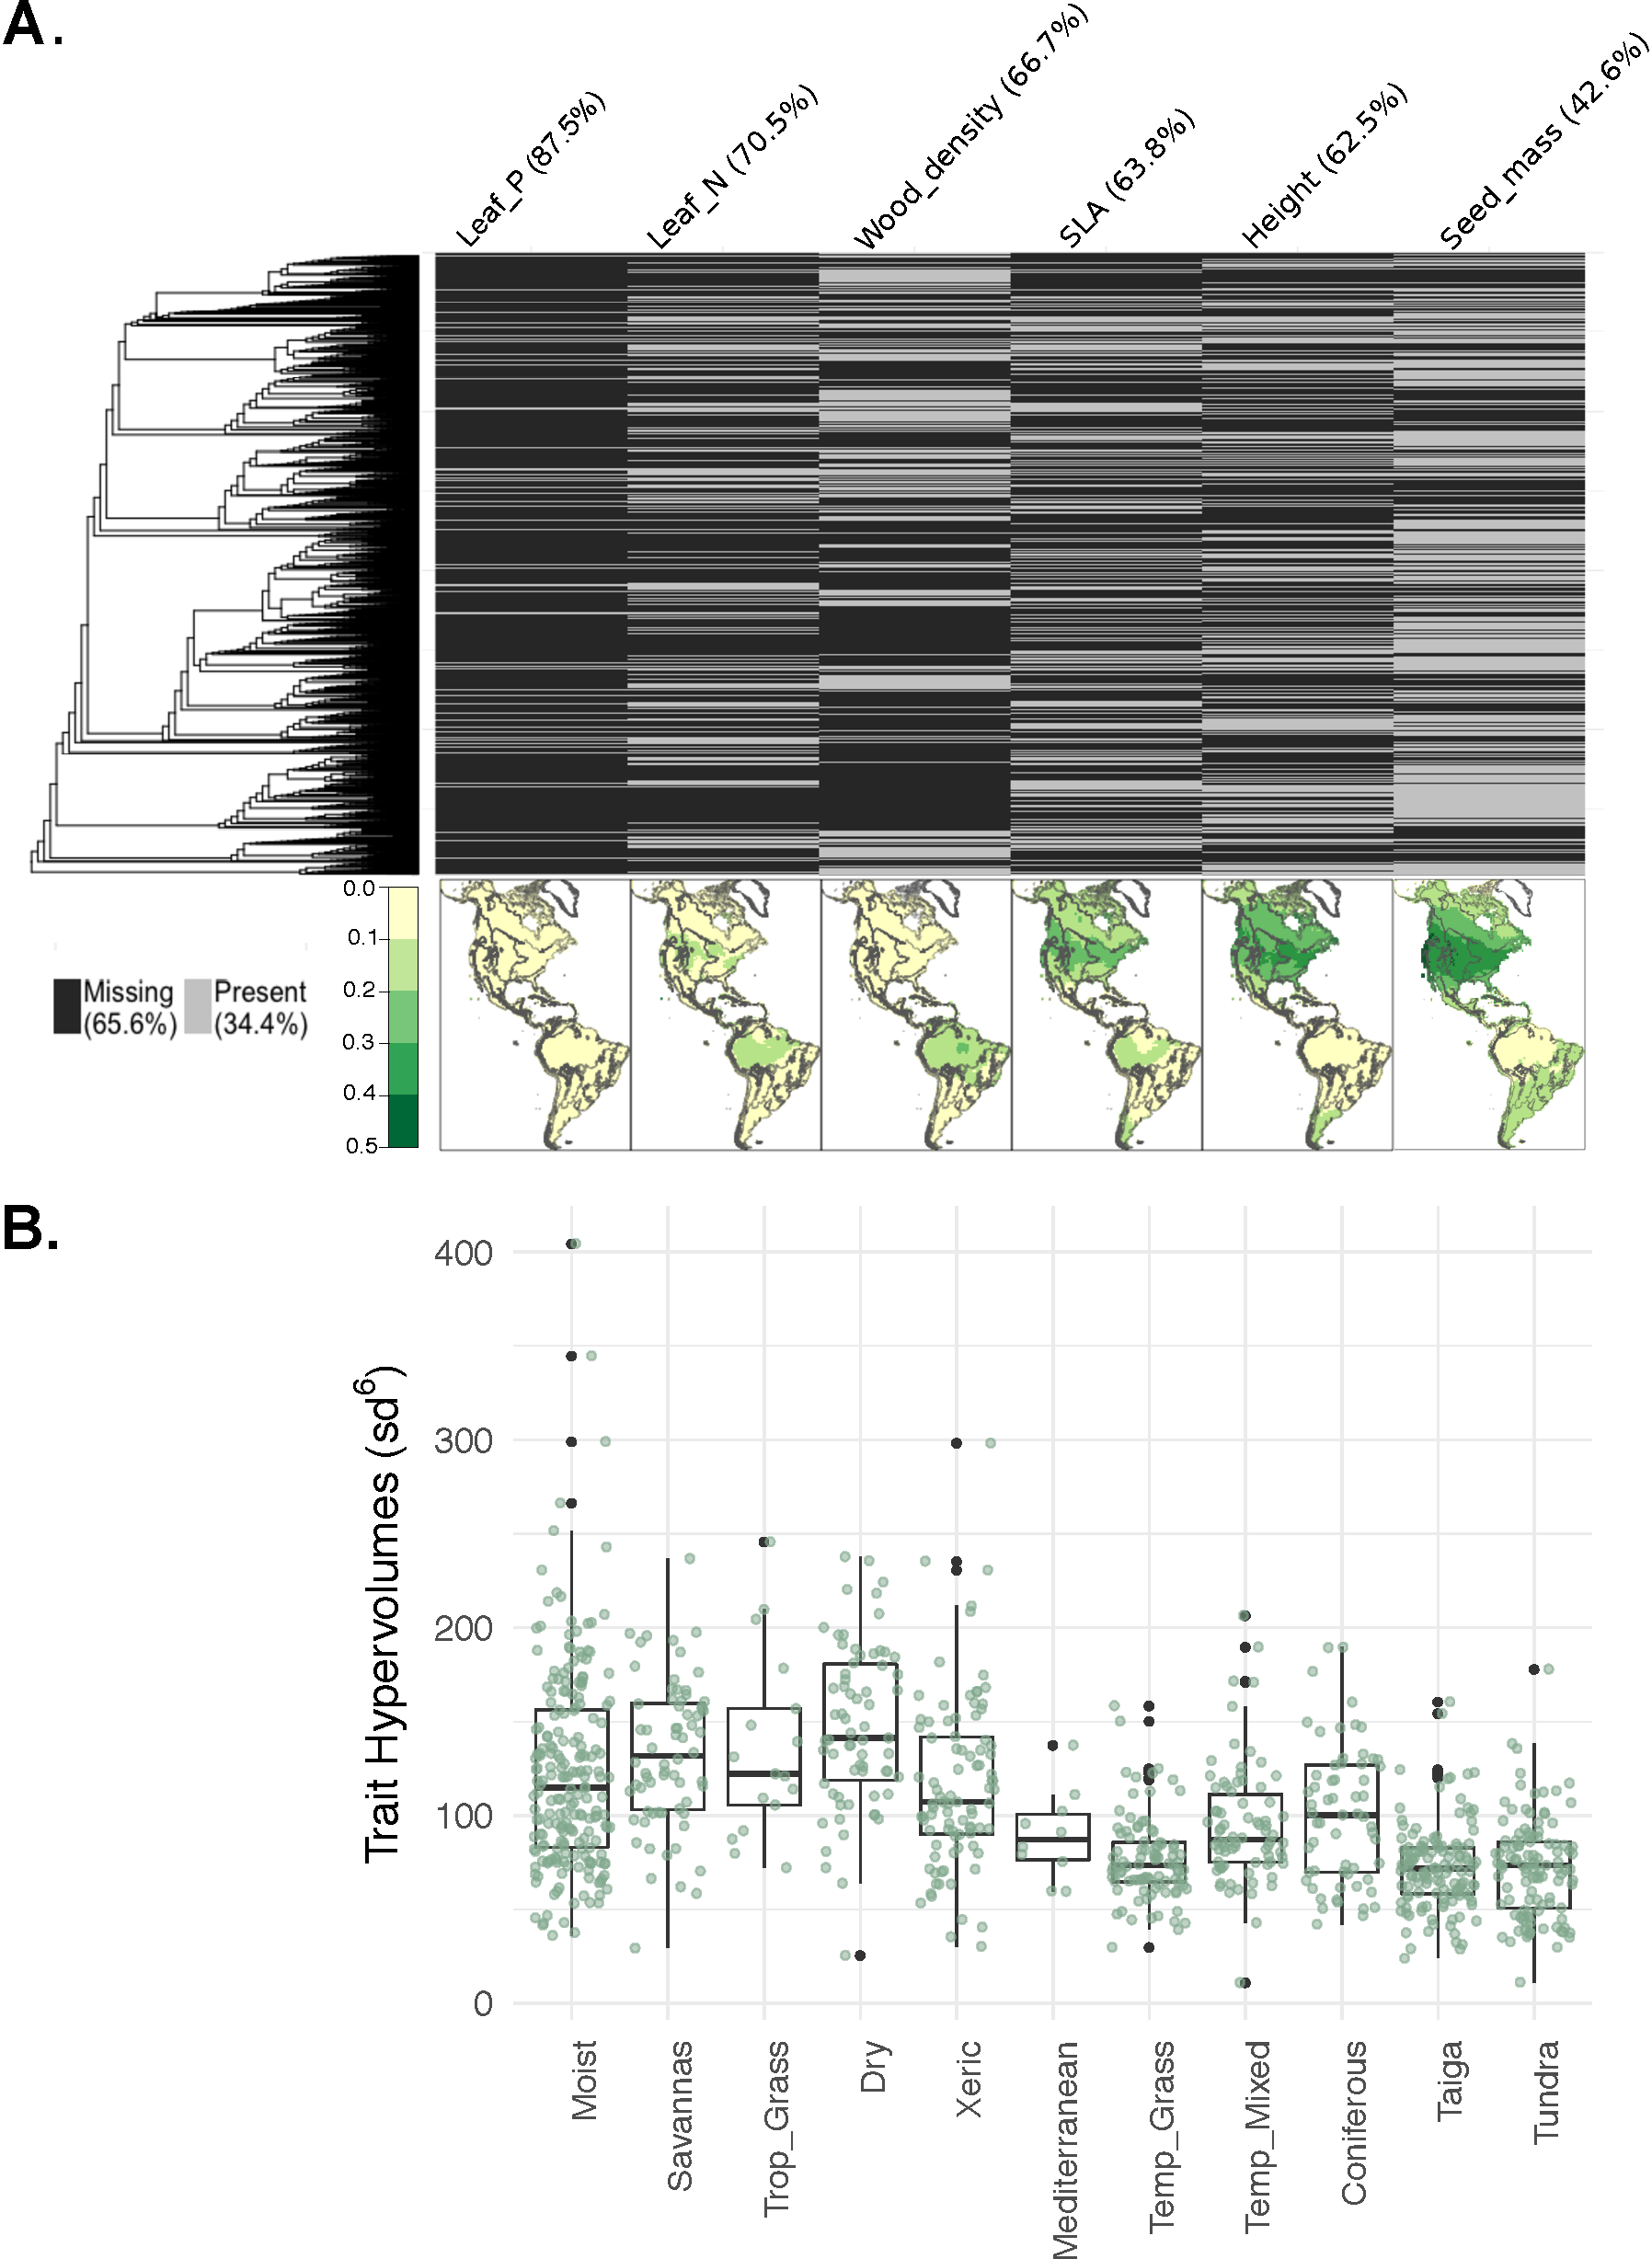
\includegraphics[scale=0.5]{./figures/Figure2.pdf}
      			%\includegraphics[scale=2]{./figures/Diversification_shifts_rate2.pdf}
      			\caption{}
      			\label{fig:sampling}
      		\end{figure}
      	
      	
      	\begin{figure}[h]
      		\centering
      		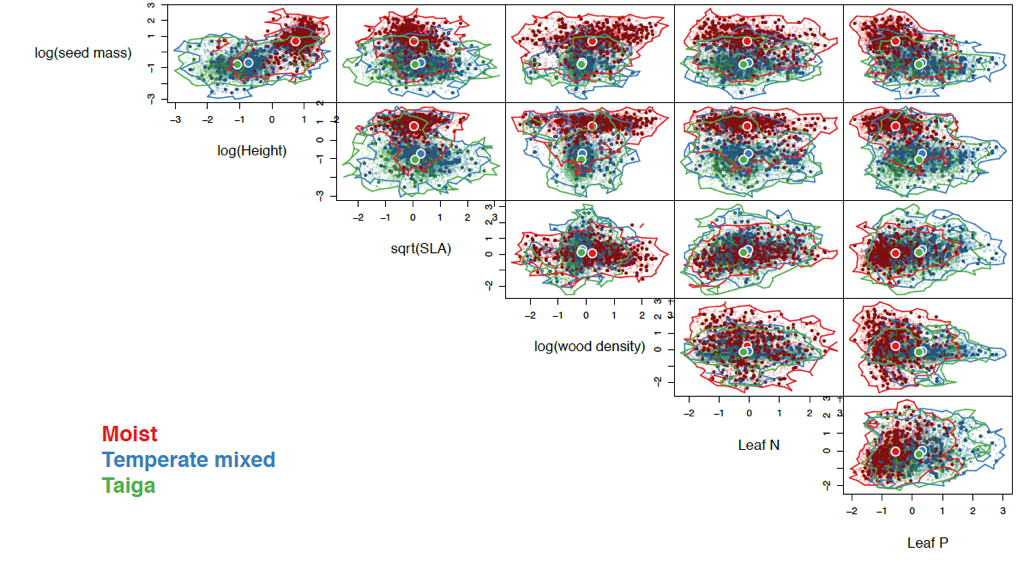
\includegraphics{./figures/Hypervolumes.png}
      		%\includegraphics[scale=2]{./figures/Diversification_shifts_rate2.pdf}
      		\caption{}
      		\label{fig:phylorate}
      	\end{figure}
      	
      		
		

    \end{column}

 
    \begin{column}{\sepwid}\end{column}			% empty spacer column
    \begin{column}{\twocolwid}							% create a two-column-wide column and then we will split it up later
      
      \vskip2.5ex
      		 \begin{figure}[h]
      	\centering
      	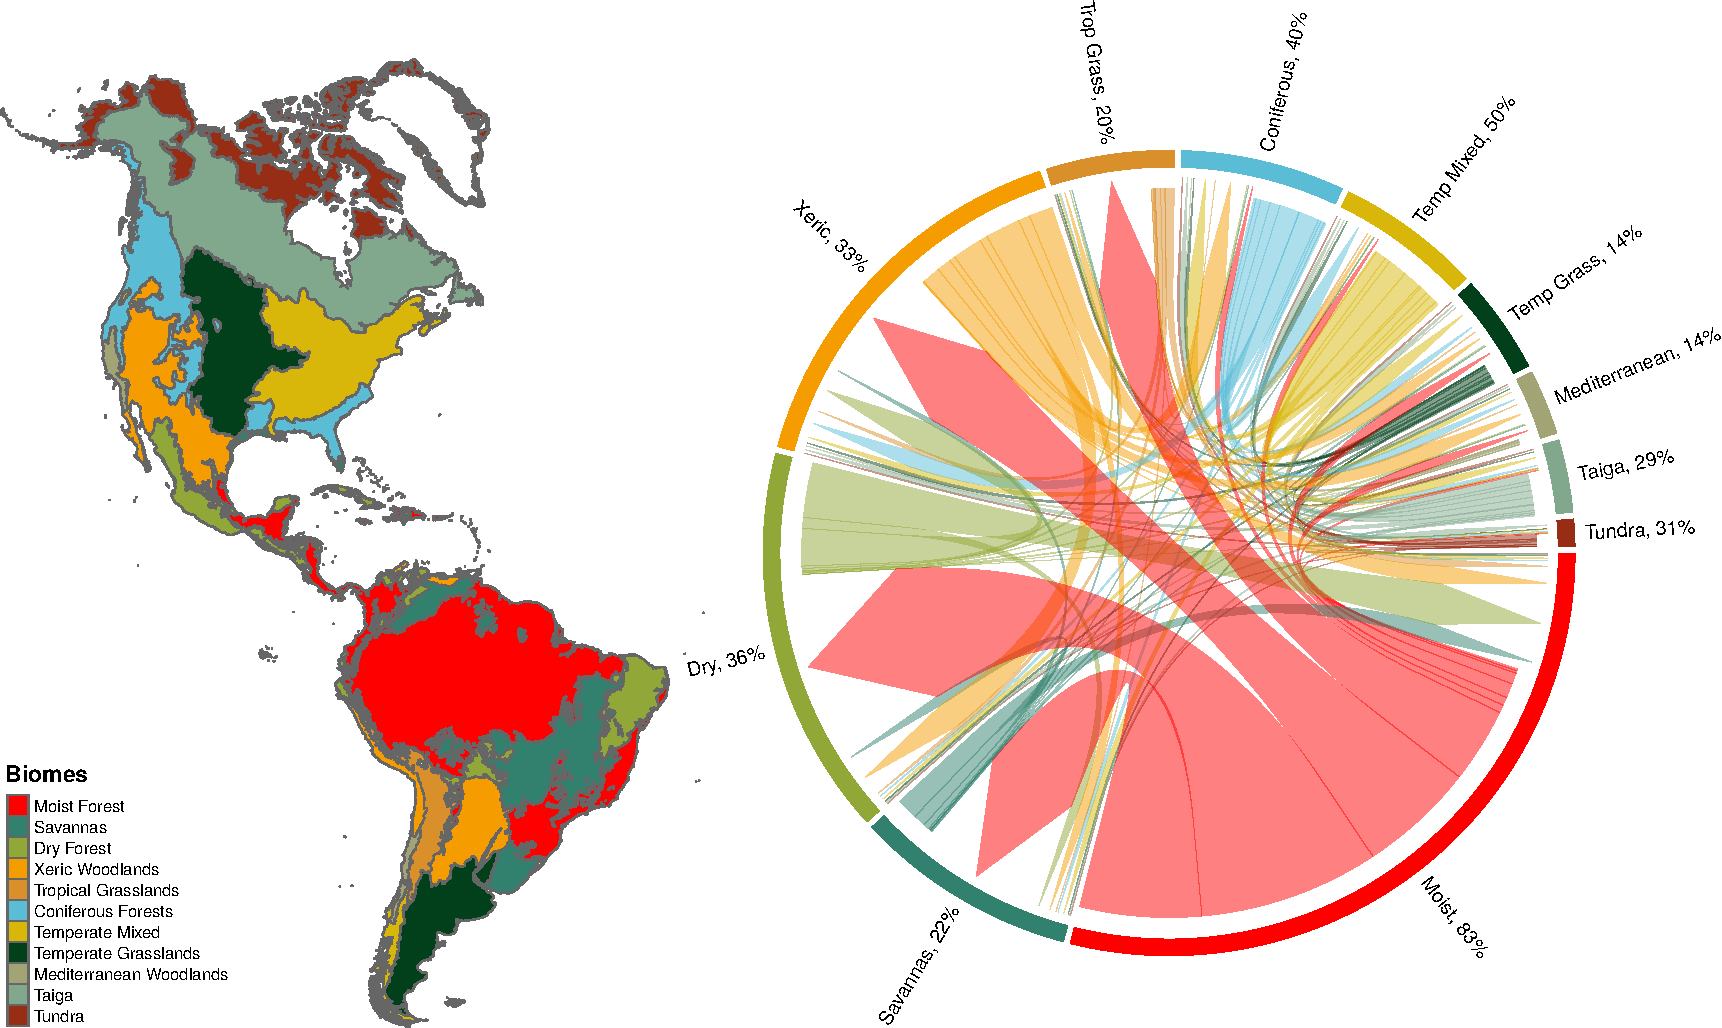
\includegraphics[width=.75\textwidth]{./figures/Figure1.pdf}
      	\caption{}
      	\label{}
	\end{figure}   


		 \begin{block}{Results}
      
		 \end{block}
 
     
 \end{column}
  

   
  \begin{column}{\sepwid}\end{column}			% empty spacer column
  \begin{column}{\onecolwid}
  
  		      		
      \begin{figure}[h]
		\centering
		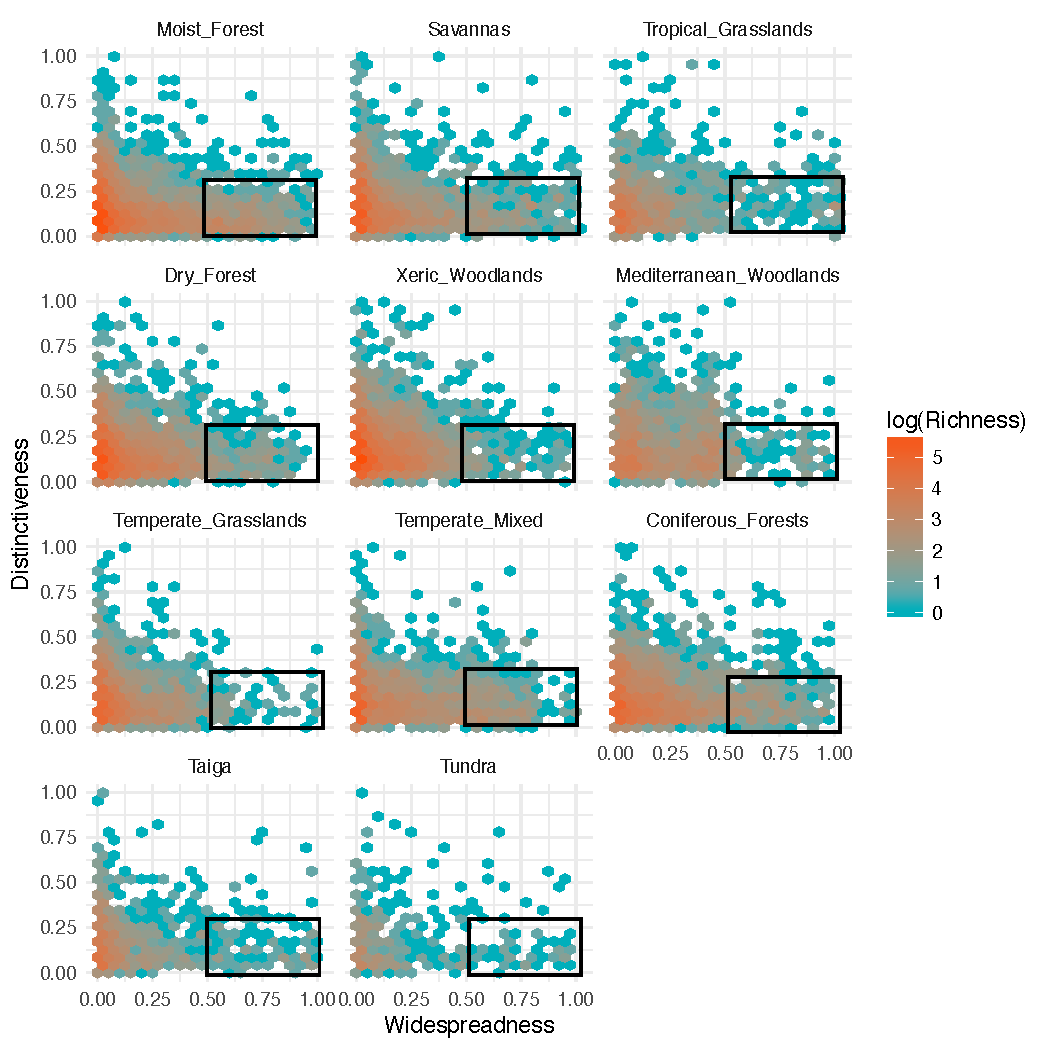
\includegraphics[scale=0.6]{./figures/Figure3.pdf}
		\caption{}
		\label{fig:rate_variation}
		\end{figure}
	
	\begin{figure}[h]
		\centering
		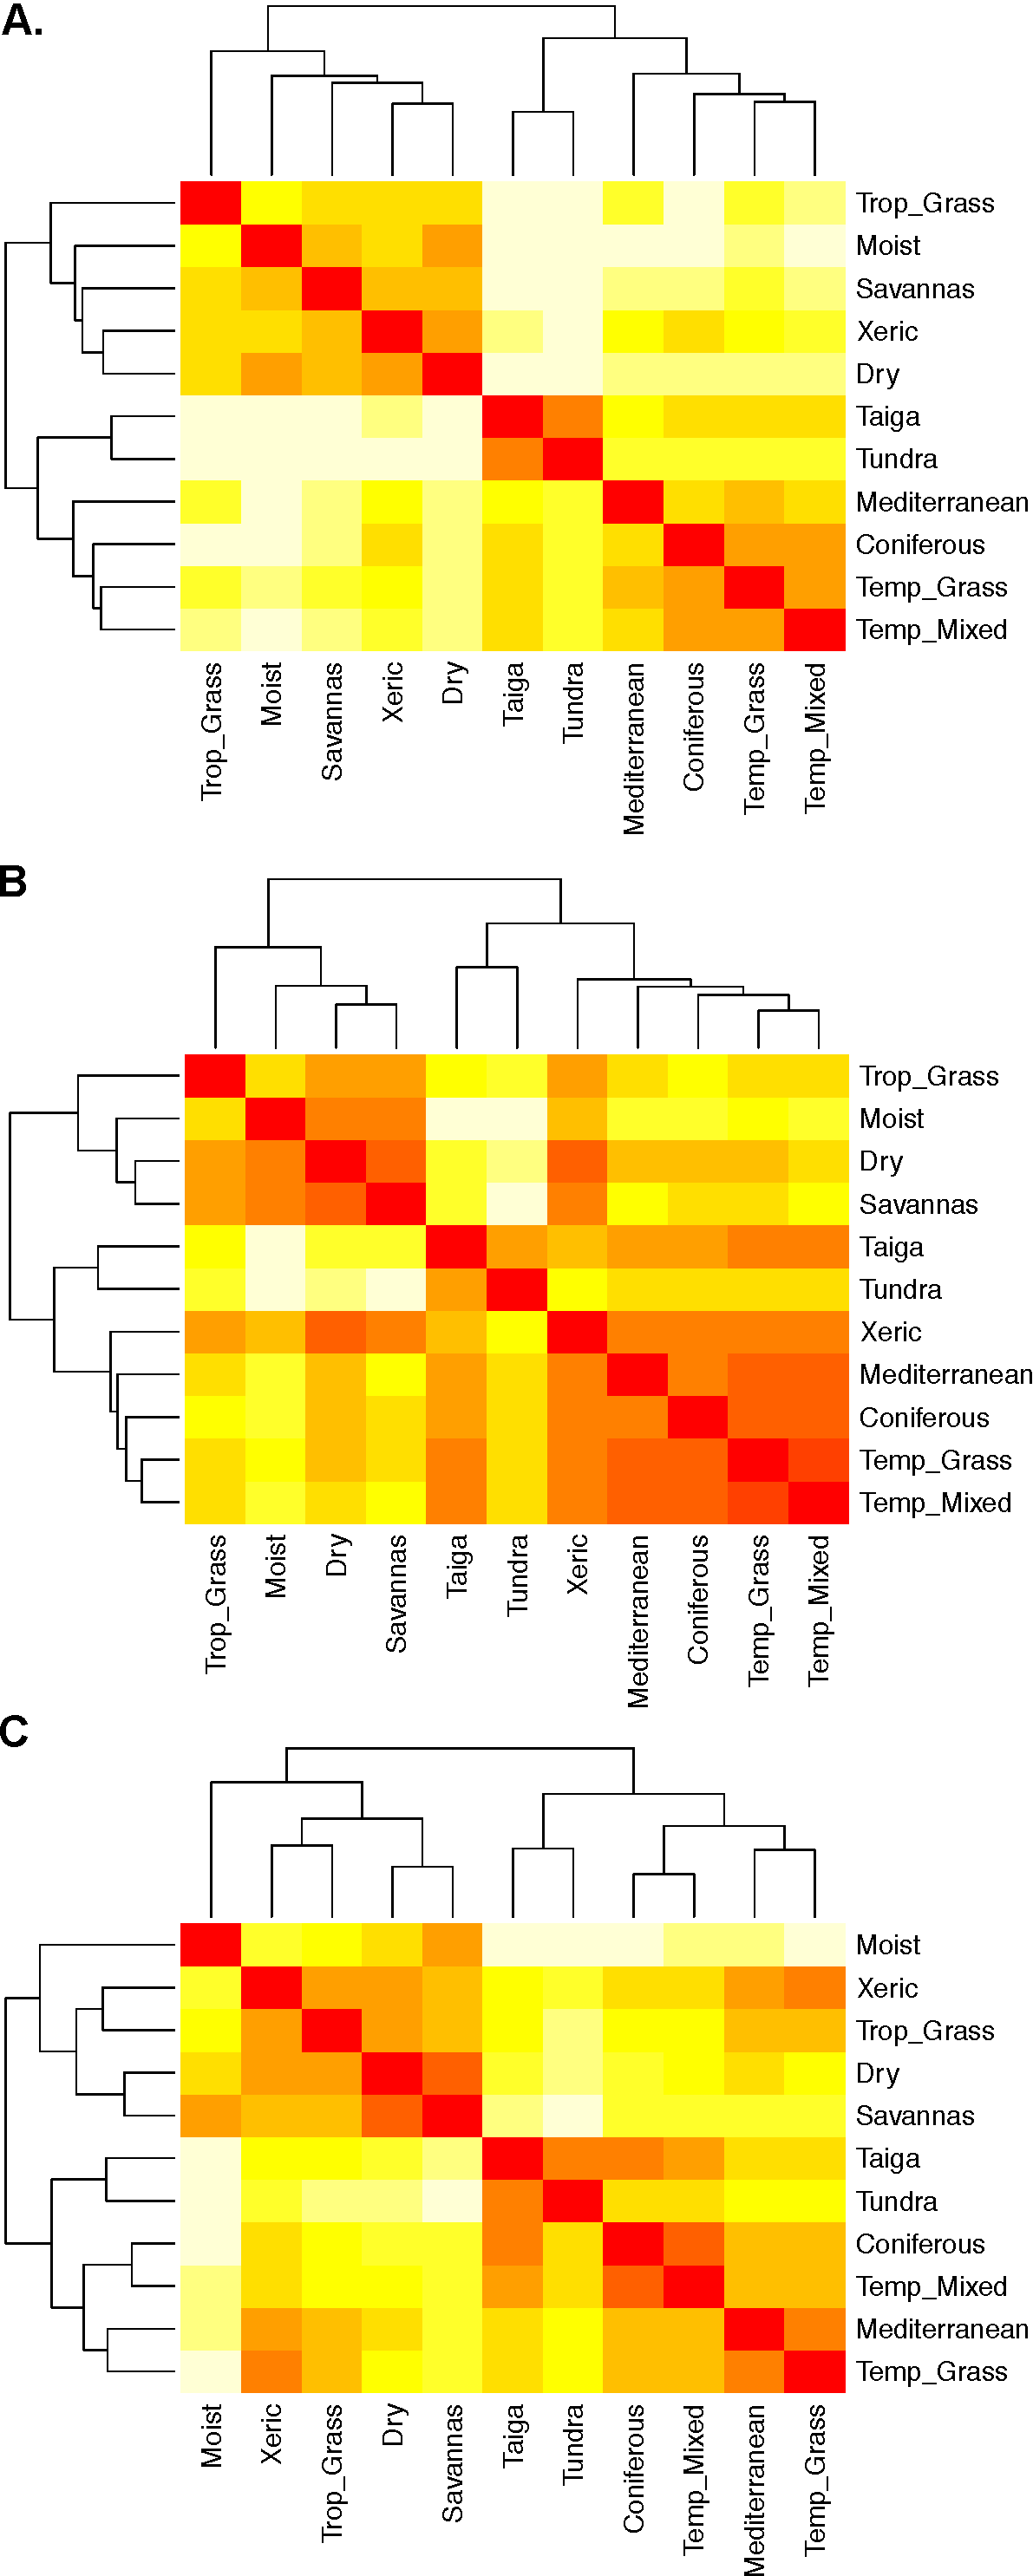
\includegraphics[scale=0.6]{./figures/Figure5.pdf}
		\caption{}
		\label{}
	\end{figure}




			\begin{block}{Discussion}
   
      		\end{block}
      		
      		\begin{block}{Next steps}

      		\end{block}
      		
      	      		
      		
    \vskip2ex
   
          		\begin{block}{References}
           	
		        \tiny{\begin{thebibliography}{99}
		        
		               	        
		        
		        \end{thebibliography}}
		        
			     \vspace{0.75in}
			      
		 		\end{block}   
		 		
		 		
      		\begin{block}{Acknowledgments}
      				
      		\end{block} 
    
    
    \vskip2ex
    
  \end{column}
  \begin{column}{\sepwid}\end{column}			% empty spacer column
 \end{columns}
\end{frame}
\end{document}
